\section{Discussion} \label{discussion}
The model that achieved the highest F1 score on the validation set were MLP neural networks. The difference in accuracy and F1 score between the validation and test set was shown to be smaller in comparison to SVMs and random forest.
The activation function `relu', known as the rectified linear unit function, was chosen. This function returns $f(x) = \max{(0,x)}$ and defines the output of a node in a hidden layer given a set of inputs. The hidden layer size was set to 2 and the maximum number of iterations the solver iterates was chosen to be 200. The solver for weight optimization is set to `lbfgs', an optimizer that belongs in the family of Quasi-Newton methods. The learning rate for scheduling weight updates is set to constant; more detail on different hyperparameters can be found in Scikit Learns documentation \cite{pedregosa2011scikit}. However, the generic layered structure of a neural network has proven to be time consuming. Additionally, this technique is considered a ``black box'' technology, and finding out why a neural network has poor performance, or how it performs the classification process, is extremely difficult \cite{noriega2005multilayer}.

\begin{figure}[ht]

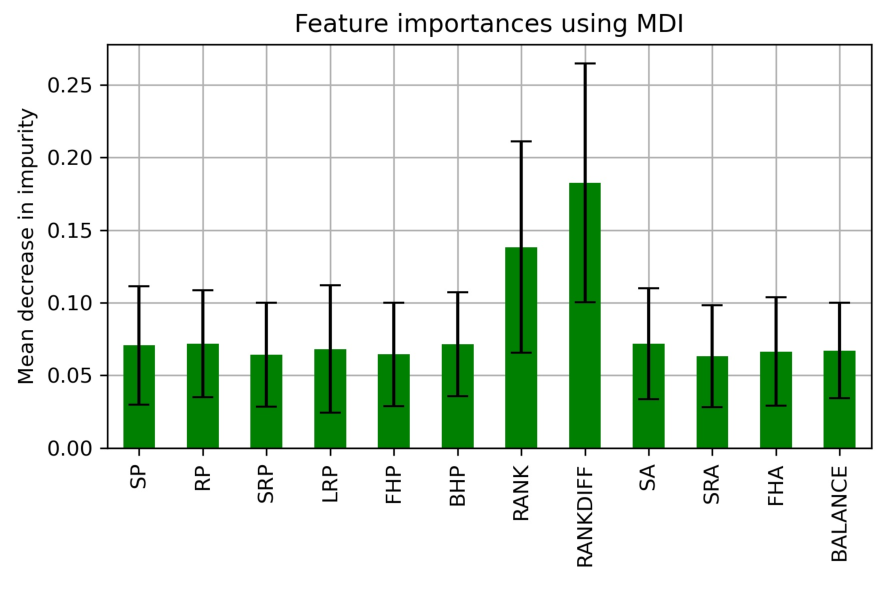
\includegraphics[width=8.5cm]{plots/feature_importance.pdf}
\caption{Importance of features from random forest classifier}

\label{fig4}
\centering
\end{figure}

One of the main advantages of using random forest is that it is much faster to train. This made tuning hyperparameters easier as training the model several times was less computationally expensive. The maximum number of levels in each decision tree was set to 80, the maximum number of features considered for splitting a node was set to 4, the minimum number of data points allowed in a leaf node was set to 4 and the number of trees that were in the classifier was set to 200.

The importance of features from a random forest classifier can also be evaluated, as shown in Figure \ref{fig4}. This is achieved by calculating the mean decrease in impurity for features across all trees, where \textit{impurity} refers to the Gini impurity index. The impurity of a node is the probability of a specific feature being classified incorrectly assuming that it is selected randomly \cite{cassidy2014calculating}.


\subsection{Ablation Study}
We can also compare accuracy and F1 score for each model that do not include newly derived features that were defined in Section \ref{engineer}. All scores are lower for models that don't use newly derived features, and accuracy score is significantly lower in SVMs compared to other models. Results of the ablation study are shown in Table \ref{results2}.

\begin{table}[ht]
\caption{Model performance with and without newly derived features}
\label{results2}
\centering
\setlength{\tabcolsep}{8pt}
\scalebox{1.05}{%
\begin{tabular}{ l|c c|c c }

\multirow{2}{4em}{Model} &
\multicolumn{2}{|c|}{With} &
\multicolumn{2}{|c}{Without} \\
\cline{2-5}
  & Acc & F1 & Acc & F1 \\

\hline \hline 
Logistic Regression & 0.699 & 0.705 & 0.631 & 0.668 \\
Random Forest & 0.677 & 0.688 & 0.661 & 0.673 \\
Support Vector Machine & & \\
$\rightarrow$ Linear & 0.696 & 0.690 & 0.556 & 0.619 \\
$\rightarrow$ RBF    & 0.700 & 0.677 & 0.500 & 0.591 \\
$\rightarrow$ Polynomial & 0.705 & 0.685 & 0.500 & 0.640\\
$\rightarrow$ Sigmoid & 0.705 & 0.690 & 0.472 & 0.642 \\
MLP Neural Network & 0.696 & 0.708 & 0.639 & 0.683\\
[1ex]
\hline
\end{tabular}}
\end{table}